\documentclass[slide05.tex]{subfiles}
\begin{document}
\begin{frame}[plain]
    \begin{center}
        \vspace{48pt}
        {\huge\bf アナログ入力装置}
    \end{center}
\end{frame}

\begin{frame}
    \frametitle{感圧センサ}
    \begin{center}
        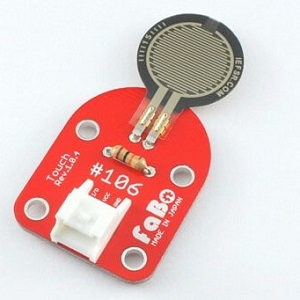
\includegraphics[width=0.4\textwidth]{../../asset/image/text05-img021.jpg}
        \begin{itemize}
            \item 加えた力の大きさの変化を測ることができる
            \item 力を加えると値が小さくなる
            \item 0〜1023の間を値をとる
        \end{itemize}
    \end{center}
    \textpageref{10}
\end{frame}

\begin{frame}
    \frametitle{ボリューム}
    \begin{center}
        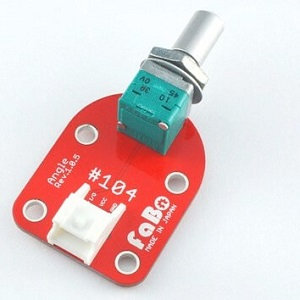
\includegraphics[width=0.4\textwidth]{../../asset/image/text05-img022.jpg}
        \begin{itemize}
            \item シャフト（じく）をひねると値の大きさを変えることができる
            \item 0〜1023の間の値をとる
            \item 左に回しきったときは変化が小さくて、右に回していくほどに変化が大きくなる（Aカーブ）
        \end{itemize}
    \end{center}
    \textpageref{10}
\end{frame}

\begin{frame}
    \frametitle{\makebox[50pt][l]{\ruby{距離}{きょ|り}センサ}}
    \begin{center}
        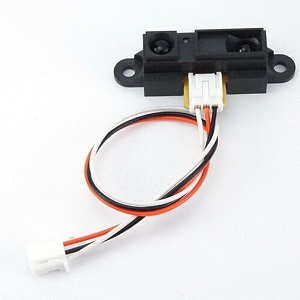
\includegraphics[width=0.4\textwidth]{../../asset/image/text05-img023.jpg}
        \begin{itemize}
            \item 距離を測ることができる
            \item 10〜80cmの距離を測ることができる
            \item ただし値は0〜1023だから、値を距離に変換しないといけない
        \end{itemize}
    \end{center}
    \textpageref{11}
\end{frame}

\begin{frame}
    \frametitle{\makebox[50pt][l]{\ruby{照度}{しょう|ど}センサ}}
    \begin{center}
        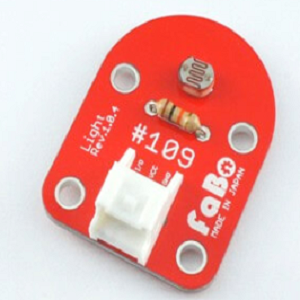
\includegraphics[width=0.4\textwidth]{../../asset/image/text05-img024.png}
        \begin{itemize}
            \item 明るさの変化を測ることができる
            \item 暗いと値が大きく、明るいと値が小さくなる
        \end{itemize}
    \end{center}
    \textpageref{11}
\end{frame}

\begin{frame}
    \frametitle{センサーをピンにつけてみよう}
    \begin{center}
        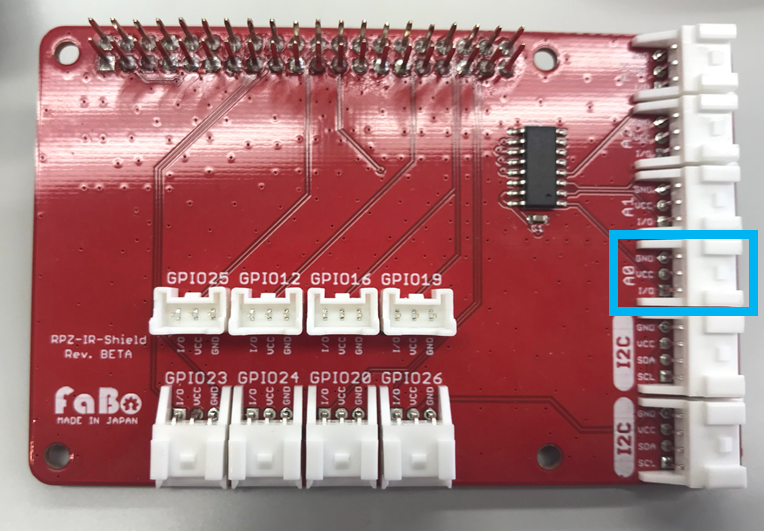
\includegraphics[width=0.8\textwidth]{../../asset/image/text05-img030.png}
        \begin{itemize}
            \item A0とアナログ入力装置をつなげてみよう
            \item HSPで\textasciitilde/05/anain.hspを動かしてみよう
        \end{itemize}
    \end{center}
    \textpageref{16}
\end{frame}

\begin{frame}[fragile]
    \frametitle{アナログ入力を使った\\プログラム}
    \begin{lstlisting}[title=\textasciitilde/05/anain.hsp]
    #include "hsp3dish.as"
    #include "rpz-gpio.as"

    spiopen 0

    *main
	    data = adcget(0,0)
	    res = "結果 : "+data+"\n"

	    redraw 0
	    pos 20,20
	    font "",30
	    mes res
	    redraw 1

	    wait 10
	    goto *main

    spiclose 0
    \end{lstlisting}
    \textpageref{16}
\end{frame}

\begin{frame}[fragile]
    \begin{exampleblock}{問題を解いてみよう}
    \begin{itemize}
        \item 教科書17ページ 問題5-7(4問)
    \end{itemize}
    \end{exampleblock}
\end{frame}
\end{document}
